
\chapter{GCSE Revision - Algebra - (Excluding Geometric problems and proofs)}
\begin{enumerate}
  \item
  \begin{enumerate}
    \item Simplify $x^7 \times x^3$\strch
    \item Simplify $(m^4)^3$\strch
    \item Simplify $\dfrac{36af^8}{12a^5f^2}$\strch\\ \vspace*{0pt}\lmrk{1}{7}
  \end{enumerate}
  \pagebreak
  \item %
  \begin{enumerate}
    \item Solve $\dfrac{4(8x - 2)}{3x} = 10$\mrk{3}\strch
    \item Write as a single fraction in its simplest form\mrk{3}
    $$
    \frac{2}{y + 3} - \frac{1}{y - 6}
    $$
    \strch
  \end{enumerate}
  %
  \item Solve the simultaneous equations
  \begin{align*}
    3x + 4y = 5\\
    2x - 3y = 9
  \end{align*}
  \hfill$x =\ $\dline\\
  \vspace*{0pt}\hfill$y =\ $\dline\\
  \vspace*{0pt}\lmrk{3}{4}
  \strch
  \item %
  \begin{align*}
    &A = 4bc\\
    &A = 100\\
    &b = 2
  \end{align*}
  \begin{enumerate}
    \item Work out the value of $c$.\mrk{2}\strch\newpage
    \item Make $k$ the subject of the formula, $m = \sqrt{\dfrac{k+1}{4}}$.\mrk{3}\strch
  \end{enumerate}
  \item Solve $\dfrac{4x - 1}{5} + \dfrac{x + 4}{2} = 3$\mrk{3}\strch\\
  \vspace*{0cm}\hfill$x =\ $\dline
  \item %
  \begin{enumerate}
    \item Simplify $a^4\times a^5$\mrk{1}\strch
    \item Simplify $\dfrac{45e^6f^8}{5ef^2}$\mrk{2}\strch
    \item Write down the value of $9^{\frac{1}{2}}$.\mrk{1}\strch
  \end{enumerate}
  \newpage
  \item Solve the simultaneous equations\mrk{6}
  \begin{align*}
    x^2 + y^2 &= 9\\
    x + y &= 2
  \end{align*}
  Give your answers correct to 2 decimal places.\strch\\
  \vspace*{0pt}\hfill$x =\ $\dline\hspace{0.2cm} $y =\ $\dline\\
  \vspace*{0pt}\hfill or $x =\ $\dline\hspace{0.2cm} $y =\ $\dline
  \item Make $p$ the subject of the formula $y = 3p^2 - 4$.\mrk{3}\strch
  \item %
  \begin{enumerate}
    \item Factorise	$6 + 9x$.\mrk{1}\strch
    \item Factorise	$y^2 - 16$.\mrk{1}\strch
    \item Factorise	$2p^2 - p - 10$.\mrk{2}\strch
  \end{enumerate}
  \newpage
  \item Solve $\dfrac{2 - y}{5} = 1$.\mrk{5}\strch\\\vspace*{0pt}\hfill $y =\ $\dline
  \item The expression $x^2 - 8x + 21$ can be written in the form $(x - a)^2 + b$ for all values of $x$.
  \begin{enumerate}
    \item Find the value of $a$ and the value of $b$.\mrk{3}\strch\\
    \vspace*{0pt}\hfill $a =\ $\dline\\
    \vspace*{0pt}\hfill $b =\ $\dline
    \suspend{enumerate}
    The equation of a curve is $y = f(x)$ where $f(x) = x^2 - 8x + 21$. The diagram shows part of a sketch of the graph of $y = f(x)$.
    \begin{figure}[H]
      \centering
      \begin{tikzpicture}
        \begin{axis}[
            xmin = -1, xmax = 10,
            ymin = -2, ymax = 30,
            xticklabels = {},
            yticklabels = {},
            axis lines = middle,
            xlabel = {$x$},
            ylabel = {$y$},
          ]
          % Plot a function
          \addplot[
            domain = -0.8:8.8,
            samples = 200,
            smooth,
            thick,
          ] {x^2 - 8*x + 21};
          \node at (7.5, 28) {$y = f(x)$};
          \node at (-0.4, -1) {$O$};
          \node at (4, 3) {$M$};
          \addplot[
            mark=x,
            mark size=6pt
          ]
          coordinates {
            (4, 5)
          };
        \end{axis}
      \end{tikzpicture}
    \end{figure}
    The minimum point of the curve is $M$.
    \resume{enumerate}
    \item Write down the coordinates of $M$.\mrk{1}\strch\\
    \vspace*{0pt}\hfill (
      \tikz\draw[thick, dashed] (0,0) -- (1.5,0);, \tikz\draw[thick, dashed] (0,0) -- (1.5,0);
    )
  \end{enumerate}
  \newpage
  \item Simplify $\dfrac{4(x + 5)}{x^2 + 2x - 15}$.\mrk{2}\strch
  \item Solve the simultaneous equations\mrk{4}
  \begin{align*}
    4x + 7y &= 1\\
    3x + 10y &= 15
  \end{align*}\strch\\
  \vspace*{0pt}\hfill$x =\ $\dline\\
  \vspace*{0pt}\hfill$y =\ $\dline
  \begin{enumerate}
    \item Solve 	$2x^2 + 9x - 7 = 0$. Give your solutions correct to 3 significant figures.\mrk{3}\strch
    \item Solve $\dfrac{2}{y^2} + \dfrac{9}{y} - 7 =0$. Give your solutions correct to 3 significant figures.\mrk{2}\strch
  \end{enumerate}
  \item Simplify $\dfrac{x + 1}{2} + \dfrac{x + 3}{3}$.\mrk{3}\strch
  \newpage
  \item %
  \begin{enumerate}
    \item %
    \begin{enumerate}
      \item Factorise $2t^2 + 5t + 2$.\strch
      \item $t$ is a positive whole number.\par
      The expression $2t^2 + 5t + 2$ can never have a value that is a prime number. Explain why.\mrk{3}\strch
    \end{enumerate}
  \end{enumerate}
  \item Make $t$ the subject of the formula\mrk{4} $$p = \frac{3-2t}{4 + t}$$\strch
  \item Solve $\dfrac{5(2x + 1)^2}{4x + 5} = 5x - 1$.\mrk{5}\strch
  \item Solve the equations\mrk{4}
  \begin{align*}
    3x + 5y &= 19\\
    4x - 2y &= -18
  \end{align*}
  \strch\\
  \vspace*{0pt}\hfill$x =\ $\dline\\
  \vspace*{0pt}\hfill$y =\ $\dline
  \item Solve the equation 	$5x^2 + 8x - 6 = 0$. Give each solution correct to 2 decimal places.\mrk{3}\strch
  \newpage
  \item %
  \begin{enumerate}
    \item On the number line below, show the inequality $-2 < y < 3$.\mrk{1}
    \begin{figure}[H]
      \centering
      \begin{tikzpicture}
        \draw[-Straight Barb, thick] (-4.5, 0) -- (5.5, 0) node[anchor=north west] {$y$};
        \foreach \x in {-4, -3, -2, -1, 0, 1, 2, 3, 4, 5}
          \draw (\x cm, 3pt) -- (\x cm, -3pt) node[anchor=north] {$\x$};
      \end{tikzpicture}
    \end{figure}\strch
    \item Here is an inequality, in $x$, shown on a number line.\mrk{2}
    \begin{figure}[H]
      \centering
      \begin{tikzpicture}
        \draw[-Straight Barb, thick] (-4.5, 0) -- (5.5, 0) node[anchor=north west] {$x$};
        \foreach \x in {-4, -3, -2, -1, 0, 1, 2, 3, 4, 5}
          \draw (\x cm, 3pt) -- (\x cm, -3pt) node[anchor=north] {$\x$};
        \draw[thick] (-3, 0.5) -- (4, 0.5);
        \filldraw[fill=white, draw=black] (-3, 0.5) circle (0.15cm);
        \fill[black] (4, 0.5) circle (0.15cm);
      \end{tikzpicture}
    \end{figure}
    Write down the inequality.\strch
    \item Solve the inequality $4t - 5 > 9$.\mrk{2}\strch
  \end{enumerate}
  \item %
  \begin{enumerate}
    \item Factorise fully $2x^2 - 4xy$.\mrk{2}\strch
    \item Factorise $p^2 - 6p + 8$.\mrk{2}\strch
    \item Simplify $\dfrac{(x+2)^2}{x+2}$.\mrk{1}\strch
    \item Simplify $2a^2b \times 3a^3b$.\mrk{2}\strch
  \end{enumerate}
  \newpage
  \item Solve $3x^2 - 4x - 2 = 0$ Give your solutions correct to 3 significant figures.\mrk{3}\strch
  \item Make $t$ the subject of the formula $2(d - t) = 4t + 7$.\mrk{3}\strch\\
  \vspace*{0pt}\hfill$t =\ $\dline
  \item %
  \begin{enumerate}
    \item Simplify fully $\dfrac{x^2 + 3x - 4}{2x^2 - 5x + 3}$.\mrk{3}\strch
    \item Write $\dfrac{4}{x + 2} + \dfrac{3}{x - 2}$ as a single fraction in its simplest form.\mrk{3}\strch
  \end{enumerate}
  \item %
  \begin{enumerate}
    \item Factorise $x^2 + px + qx + pq$.\mrk{2}\strch
    \item Factorise $m^2 - 4$.\mrk{1}\strch
    \item Write as a single fraction in its simplest form $\dfrac{2}{x - 4} - \dfrac{1}{x + 3}$.\mrk{3}\strch
  \end{enumerate}
  \newpage
  \item Find the exact solutions of $x + \dfrac{3}{x} = 7$.\mrk{3}\strch
  \item 	$-2 \leq n < 5$, $n$ is an integer.
  \begin{enumerate}
    \item Write down all the possible values of $n$.\mrk{2}\strch
    \item Solve the inequality	$4x + 1 > 11$.\mrk{2}\strch
  \end{enumerate}
  \item Simplify $(2n^3)^4$.\mrk{2}\strch
  \item %
  \begin{enumerate}
    \item Factorise $2x^2 - 9x + 4$.\mrk{2}\strch\\
    Hence, or otherwise,
    \item Solve $2x^2 - 9x + 4 = (2x - 1)^2$\mrk{4}\strch
  \end{enumerate}
  \newpage
  \item $y = p - 2qx^2$\par
  $p = -10,\quad q = 3,\quad	x = -5$    
  \begin{enumerate}
    \item Work out the value of $y$.\mrk{2}\strch
    \item Rearrange $y = p - 2qx^2$ to make $x$ the subject of the formula.\mrk{3}\strch
  \end{enumerate}
  \item The diagram shows the graph of $y = x^2 - 5x - 3$
  \begin{figure}[H]
    \centering
    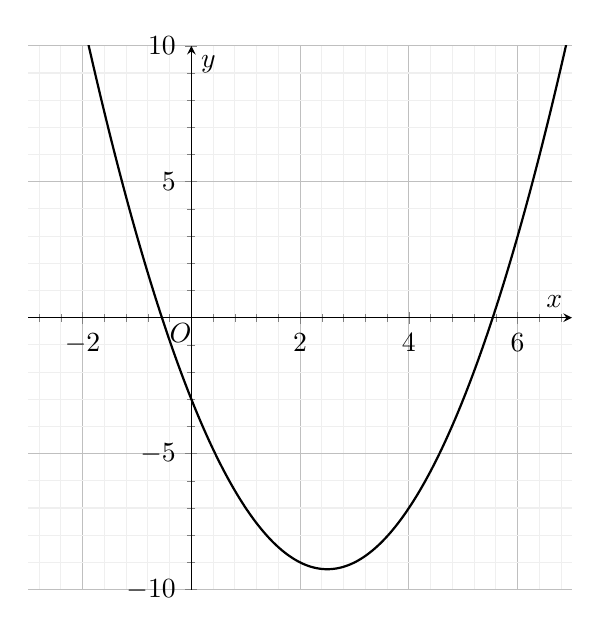
\begin{tikzpicture}
      \begin{axis}[
          xmin = -3, xmax = 7,
          ymin = -10, ymax = 10,
          grid = both,
          minor tick num = 4,
          major grid style = {lightgray},
          minor grid style = {lightgray!25},
          axis lines = center,
          width = 0.7\textwidth,
          height = 0.7\textwidth,
          xlabel = {$x$},
          ylabel = {$y$},
        ]
        % Plot a function
        \addplot[
          domain = -2:7,
          samples = 500,
          smooth,
          thick,
        ] {x^2 - 5*x - 3};
        \node at (-0.2, -0.55) {$O$};
      \end{axis}
    \end{tikzpicture}
  \end{figure}
  \newpage
  \begin{enumerate}
    \item Use the graph to find estimates for the solutions of.\mrk{3}
    \begin{enumerate}
      \item $x^2 - 5x - 3 = 0$.\strch
      \item $x^2 - 5x - 3 = 6$.\strch
    \end{enumerate}
    \item Use the graph to find estimates for the solutions of the simultaneous equations\mrk{3}
    \begin{align*}
      y &= x2 - 5x - 3\\
      y &= x - 4
    \end{align*}\strch
  \end{enumerate}
  \item The table shows six expressions. $n$ is a positive integer.\par
  \begin{table}[H]
    \centering
    \resizebox{0.85\textwidth}{!}{%
    \begin{tabular}{|c|c|c|c|c|c|} 
      \hline
      $2n - 3$ & $3n - 2$ & $3(n + 4)$ & $4n + 1$ & $4(3n + 1)$ & $2n + 1$ \\ 
      \hline
    \end{tabular}}
  \end{table}
  \begin{enumerate}
    \item From the table, write the expression whose value is\mrk{2}
    \begin{enumerate}
      \item always even.
      \item always a multiple of 3.
    \end{enumerate}
    \item From the table, write the expression which is a factor of $4n^2 - 1$.\mrk{1}\strch
  \end{enumerate}
  \item Solve the equation $\dfrac{x}{2} - \dfrac{2}{x + 1} = 1$.\mrk{4}\strch
  \newpage
  \item Make $k$ the subject of the formula $t = \dfrac{k}{k - 2}$.\mrk{4}\strch
  \item %
  \begin{enumerate}
    \item Simplify completely $\dfrac{12xy^3}{3x^2y^3}$.\mrk{2}\strch
  \end{enumerate}
  \item %
  \begin{enumerate}
    \item Expand and simplify $(2x + 4y)(4x - 5y)$.\mrk{2}\strch
    \item Simplify fully $\dfrac{(x + 10)^5}{(x + 10)^4}$.\mrk{1}\strch
    \item Simplify fully $\dfrac{x^2 - 25}{x^2 + 7x + 10}$\mrk{3}\strch
    \item For all values of $x,\ x^2 + 6x - 2 = (x + p)^2 + q$. Find the value of $p$ and the value of $q$.\mrk{3}\strch\\
    \vspace*{0pt}\hfill $p=\ $
      \tikz\draw[thick, dashed] (0,0) -- (1.5,0);, $q=\ $ \tikz\draw[thick, dashed] (0,0) -- (1.5,0);
  \end{enumerate}
  \newpage
  \item Make $v$ the subject of the formula $t = \dfrac{v}{5} + 2$.\mrk{2}\\[2cm]
  \vspace*{0pt}\hfill $v=\ $\dline
\end{enumerate}